% A template for an Honours Thesis in English Language, NUS: adapted from one by Derek Lim (2016), itself adapted from a template for Carleton College comps papers by Andrew Gainer-Dewar (2013). 
% This work is licensed under the Creative Commons Attribution 4.0 International License.
% To view a copy of this licence, visit http://creativecommons.org/licenses/by/4.0/ or send a letter to Creative Commons, 444 Castro Street, Suite 900, Mountain View, California, 94041, USA.
\documentclass[twoside]{memoir}
\usepackage{nus-el-ht}

% The Latin Modern font is a modernised replacement for the classic Computer Modern. Feel free to replace this with a different font package.
\usepackage{lmodern}
% Hyperref enables click-through hyperlinks in your PDF. The hyphens option indicates where to break long URLs. 
\PassOptionsToPackage{hyphens}{url}\usepackage{hyperref}
% We use setspace to implement double-spacing, but with a specific command to leave quotes single-spaced. 
\DisemulatePackage{setspace}\usepackage{setspace}
\expandafter\def\expandafter\quote\expandafter{\quote\singlespacing}
	\doublespacing

% Linguistics-specific packages.
% For typing IPA.
\usepackage{tipa} 
	\newcommand{\phonem}[1]{\textipa{/#1/}}
	\newcommand{\phonet}[1]{\textipa{[#1]}}
% For drawing syntax trees.
\usepackage{qtree}\usepackage{tikz} 
\usepackage{tikz-qtree}
	\tikzset{every tree node/.style={align=center,anchor=north}}
% For typesetting and labelling examples, incl. glossed examples. 
\usepackage{expex} 
	\lingset{Everyex=\singlespace}

% Titling commands. 
\title{Specification and Refinement in the Network Stack} % TODO: come up with better title
\author{Daniel Neshyba-Rowe}
\supervisor {Alain K{\"a}gi}
\degree{Bachelor of Arts with Honours}
\faculty{Mathematical Sciences faculty} % TODO: figure out if this is right
\dept{Computer Science} % TODO: should this be CS and Math?
% \date % TODO: set date?

\begin{document}
% First, we go into "front matter" mode.
% Among other things, this gives us Roman page numbers.
\frontmatter

% We tell LaTeX to make a title page, sections for acknowledgements, the abstract, and the table of contents (important!). 

\maketitle

\chapter{Acknowledgement}
`This page is for making acknowledgements that have a direct bearing on the HT and is not for indulging in routine gestures of politeness or sentimental attitudinising. In all things, the candidate should be guided by good taste and good sense' \pgcitep{ell-ht-format}{2}. % Note also the command for citing a source and a page number. 

\begin{abstract}
  % citations look like \citep{ell-ht-format}.
        Prior work led to the first proven-reliable and viable microkernel, seL4.
      We hypothesize that similar reliability is possible for a performant IoT device.
      As a proof of concept, we are creating a networked fish tank thermometer
      with a complete IPv6 network stack and formally verifying all components.

\end{abstract}

\tableofcontents

% Include the list of figures and list of tables only if you actually have figures and tables! (The * after each indicates that it should not be included in the table of contents.)
%\listoffigures*
%\listoftables*

% Next, we go into "main matter" mode.
% This resets the page numbers and uses Arabic numerals.
\mainmatter

\chapter{Introduction}

This is a chapter.

\section{Overview}

You can embed sections and subsections.

\subsection{Research Question}

Is `\LaTeX' pronounced \phonet{let\super hEk\super h} or \phonet{lat\super hEk\super h}?


\section{Trees and Glosses}

Packages have documentation that explain (among other things) how to implement them. These are brief implementation examples for \texttt{expex} and \texttt{tikz-qtree}. 

Glossed examples data can be presented like in (\ref{ex:missile}) below.

\ex\label{ex:missile}
\begingl
\gla Missile cannot anyhow tzua one. //
\glb Missile cannot carelessly fire \textsc{attr} //
\glft `Missiles should not be carelessly fired.' //
\endgl
\xe

A syntax tree can be presented and labelled as a figure, as with Figure \ref{fig:ticket-topic} below. 

\begin{figure}[h!]
\caption{Deriving `Ticket you got?' through topicalization}
\centering
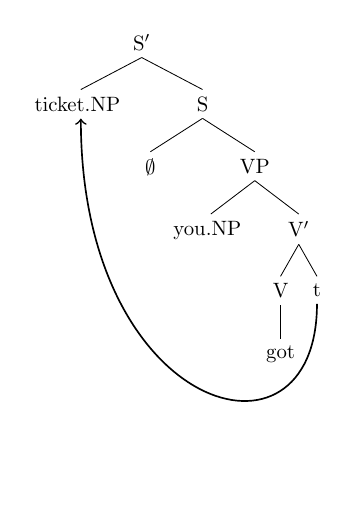
\begin{tikzpicture}[scale=0.75]
\Tree [.S$'$ \node(x){\qroof{ticket}.NP }; [.S $\emptyset$ [.VP {\qroof{you}.NP } [.V$'$ [.V got ] \node(y){t}; ] ] ] ]
\draw[semithick, <-] (x.south)..controls +(south:5) and +(south:3)..(y.south);
\end{tikzpicture}
\label{fig:ticket-topic}
\end{figure}


% If you want to include appendices, just use the \appendix command and then make chapters as normal
\appendix
\chapter{Your first appendix}

See \url{https://www.overleaf.com/read/qyhckhfyfvmb} on Overleaf for useful examples of formatted text, typing in IPA, etc.

% For the bibliography style, I load `sp.bst', the style used by the LSA in the journal `Semantics and Pragmatics'. For how to include in-line citations with page numbers and other conventions, refer to nus-el-ht.sty. 
\backmatter
\bibliography{el-ht.bib}
\end{document}
